\newpage
\section{Training our own models.} \label{training}
\subsection{Data sets}
In the following we will use two different datasets. 1) \emph{Caltech} \footnote{Available at \footnote{http://www.vision.caltech.edu/html-files/archive.html}} which consists of "450 frontal face images of 27 or so unique people." and 2) \emph{FFHQ}\footnote{Available at \footnote{https://github.com/NVlabs/ffhq-dataset}} Here we use the 5000 of the provided thumbnails of resolution 128x128.

The FFHQ dataset is already preprocessed such that the faces are aligned and the images are of the same dimensions. For Caltech however we need to do this preprocessing manually.

In the Github repository for this project we provide code to download both datasets with additional preprocessing of the Caltech dataset.

% We use OpenCVs implementation of the haarcascade to make bounding boxes around the

In Figure \ref{rawdata} we see a random sample of the processed images from the Caltech \ref{raw-caltech} and FFHQ \ref{raw-ffhq} datasets respectively.

\begin{figure}[h!]
    \centering
    \begin{subfigure}[b]{0.45\textwidth}
        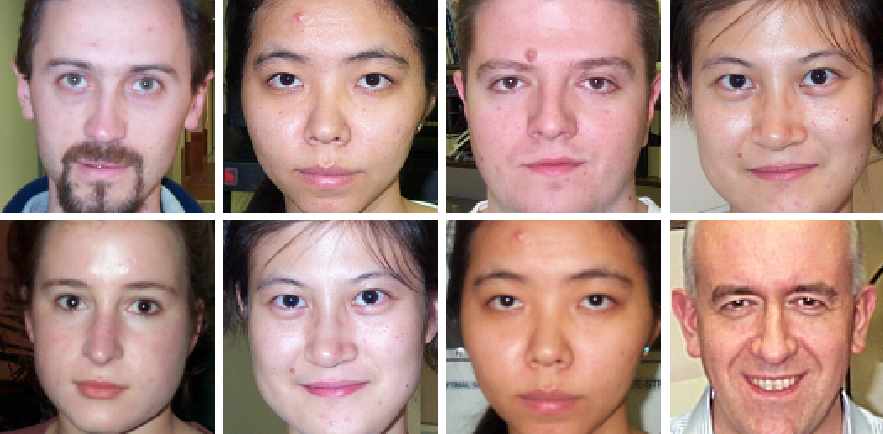
\includegraphics[width=\textwidth]{fig/data/caltech}
        \caption{Caltech dataset}
        \label{raw-caltech}
    \end{subfigure}
    ~
    \begin{subfigure}[b]{0.45\textwidth}
        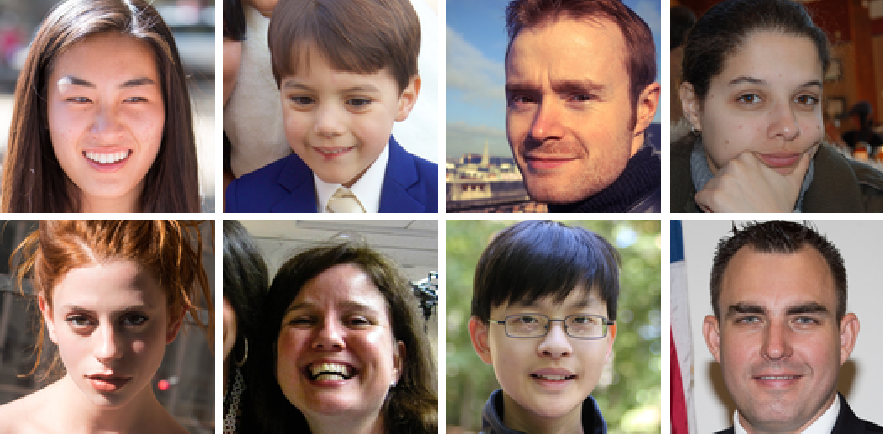
\includegraphics[width=\textwidth]{fig/data/ffhq}
        \caption{FFHQ dataset}
        \label{raw-ffhq}
    \end{subfigure}

    \caption{The raw data from the Caltech and FFHQ datasets respectively. This figure is the only one containing images of real people in the report.}
    \label{rawdata}
\end{figure}


\subsection{Principal Component Analysis }

In Figure \ref{eigenface} we see the first 8 eigenfaces.

\begin{figure}
  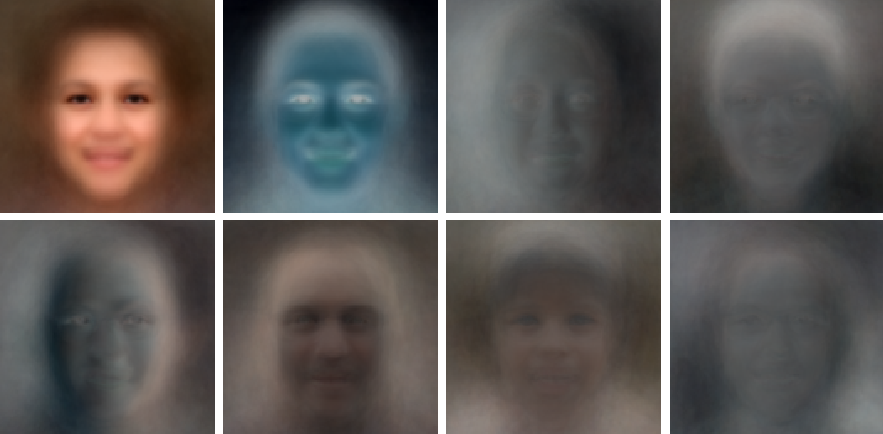
\includegraphics[width=\textwidth]{fig/PCA/pca}
  \caption{Eigenfaces of the FFHQ dataset.}
  \label{eigenface}
\end{figure}

We see that the PCA algorithms is able we capture meaningfull aspect of the dataset.

By visual inspection we observe that it seems that the Principal Components control aspects of 1) and 2) Color 3) direction of lighting 4) age 5) pose and 6) gender.

in Figure \ref{pca-components} we see the results of varying the first six
principal components.


\subsection{VAE}





\subsection{DCGAN}
In figure \ref{dcgan-results} we see the results from training a DCGAN the FFHQ and Caltech datasets for 10000 epochs.

The training time was about 6 hours in using Google Colab. As we see in the figure the result is no nowhere near photorealism.

\begin{figure}[h!]
    \centering
    \begin{subfigure}[b]{0.45\textwidth}
        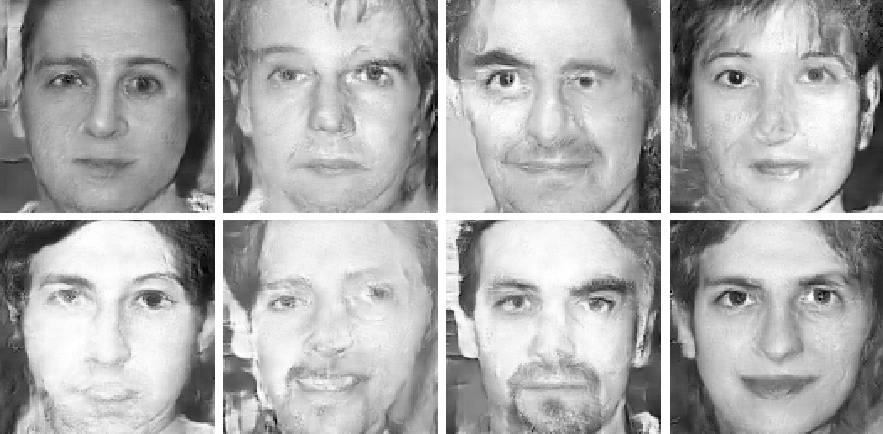
\includegraphics[width=\textwidth]{fig/dcgan/caltech/epoch10000}
        \caption{Caltech dataset B/W}
        \label{dcgan-caltech}
    \end{subfigure}
    ~
    \begin{subfigure}[b]{0.45\textwidth}
        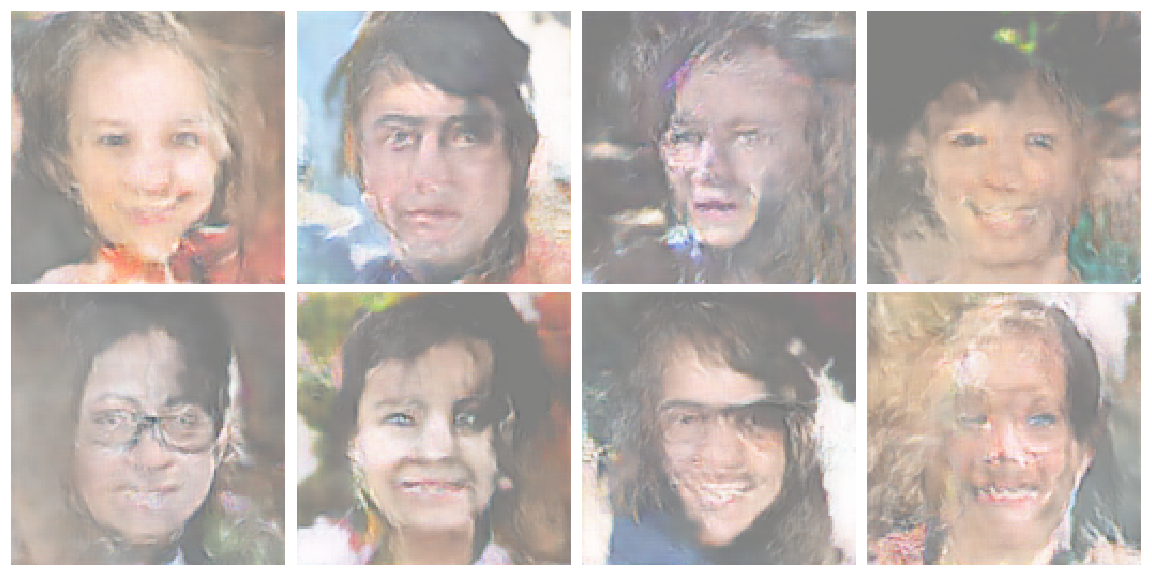
\includegraphics[width=\textwidth]{fig/dcgan/ffhq/epoch10000}
        \caption{FFHQ dataset}
        \label{dcgan-ffhq}
    \end{subfigure}
    \caption{The results from training the DCGAN for 10000 epochs on the FFHQ and Caltech datasets respectively.}
    \label{dcgan-results}
\end{figure}



% \begin{figure}
%     \centering
%     \begin{subfigure}[b]{0.3\textwidth}
%         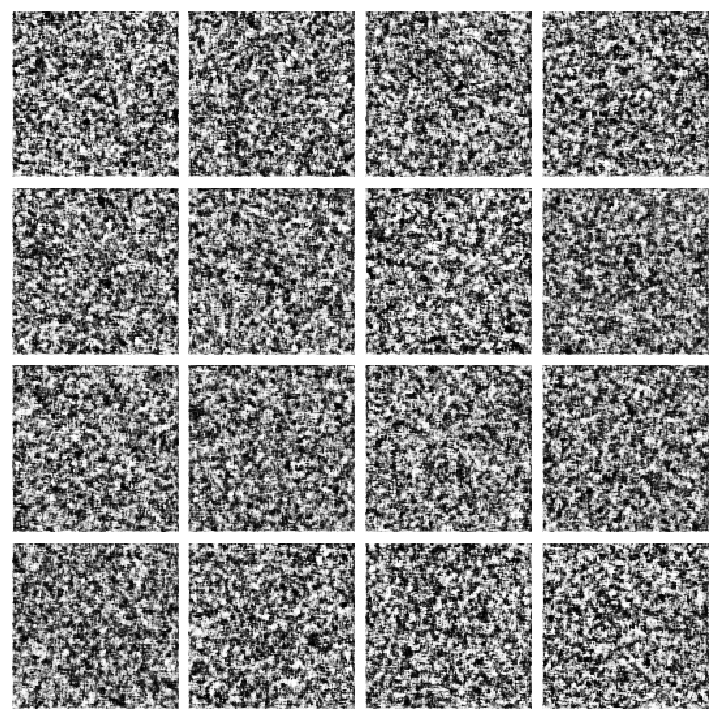
\includegraphics[width=\textwidth]{fig/dcgan/epoch0}
%         \caption{Epoch 0}
%     \end{subfigure}
%     ~
%     \begin{subfigure}[b]{0.3\textwidth}
%         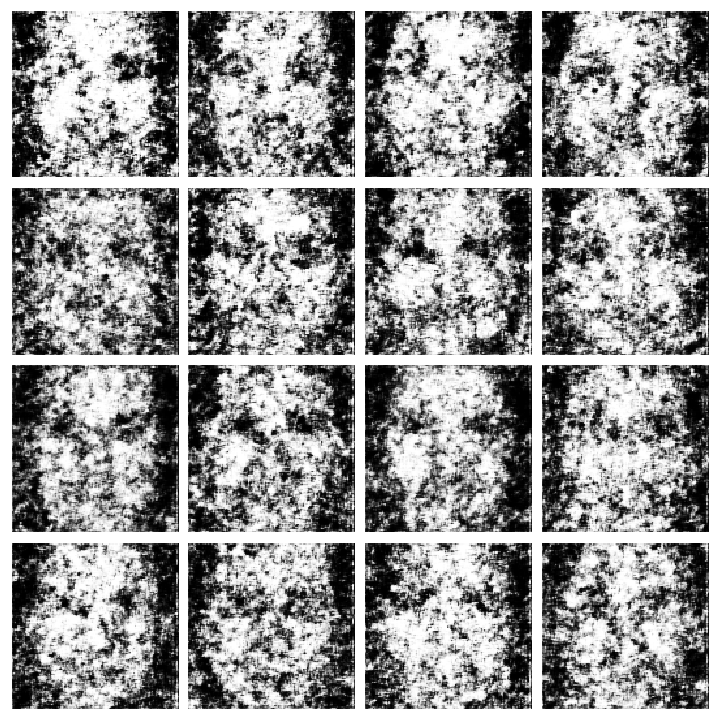
\includegraphics[width=\textwidth]{fig/dcgan/epoch10}
%         \caption{Epoch 10}
%     \end{subfigure}
%     ~
%     \begin{subfigure}[b]{0.3\textwidth}
%         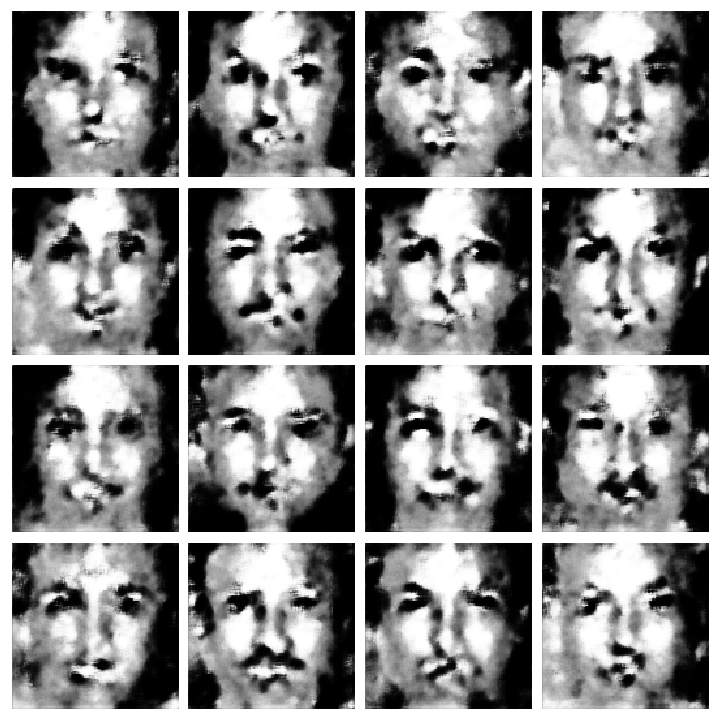
\includegraphics[width=\textwidth]{fig/dcgan/epoch100}
%         \caption{Epoch 100}
%     \end{subfigure}
%
%     \begin{subfigure}[b]{0.3\textwidth}
%         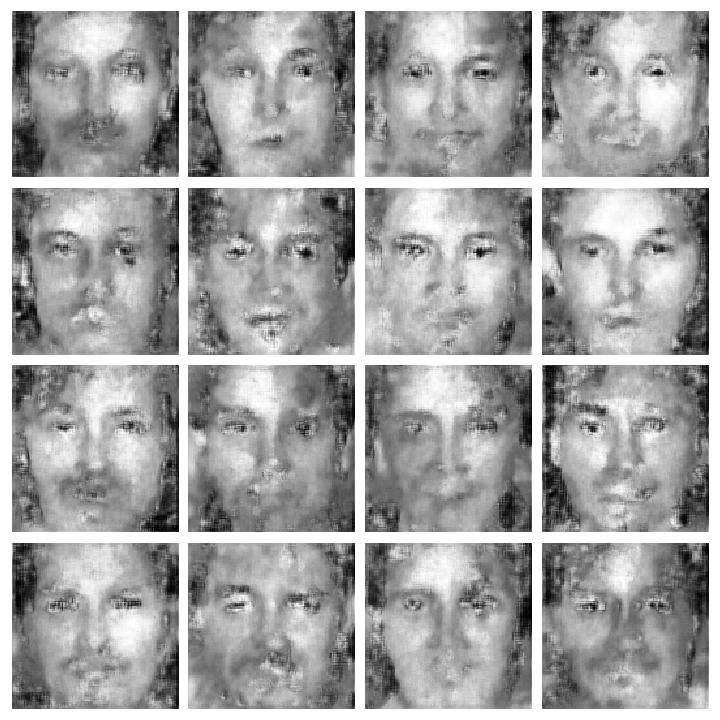
\includegraphics[width=\textwidth]{fig/dcgan/epoch200}
%         \caption{Epoch 200}
%     \end{subfigure}
%     ~
%     \begin{subfigure}[b]{0.3\textwidth}
%         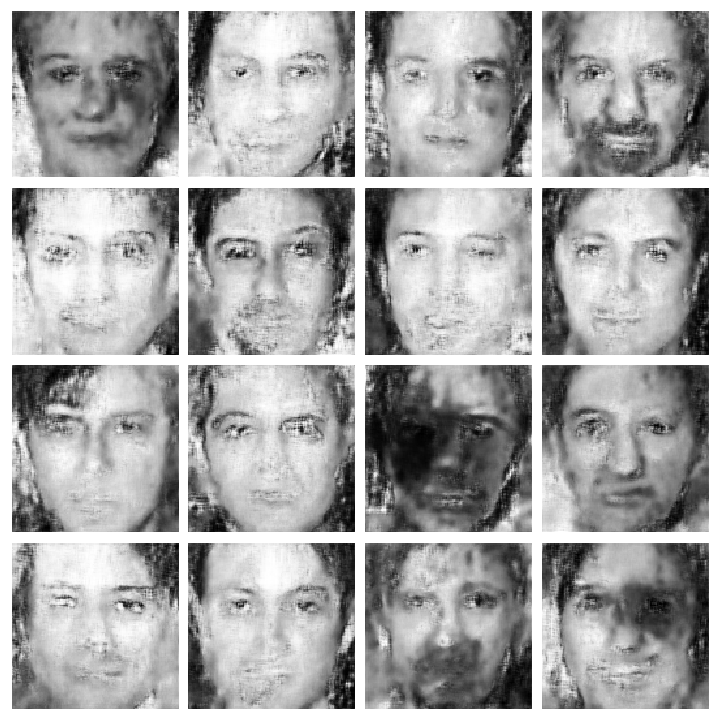
\includegraphics[width=\textwidth]{fig/dcgan/epoch400}
%         \caption{Epoch 400}
%     \end{subfigure}
%     ~
%     \begin{subfigure}[b]{0.3\textwidth}
%         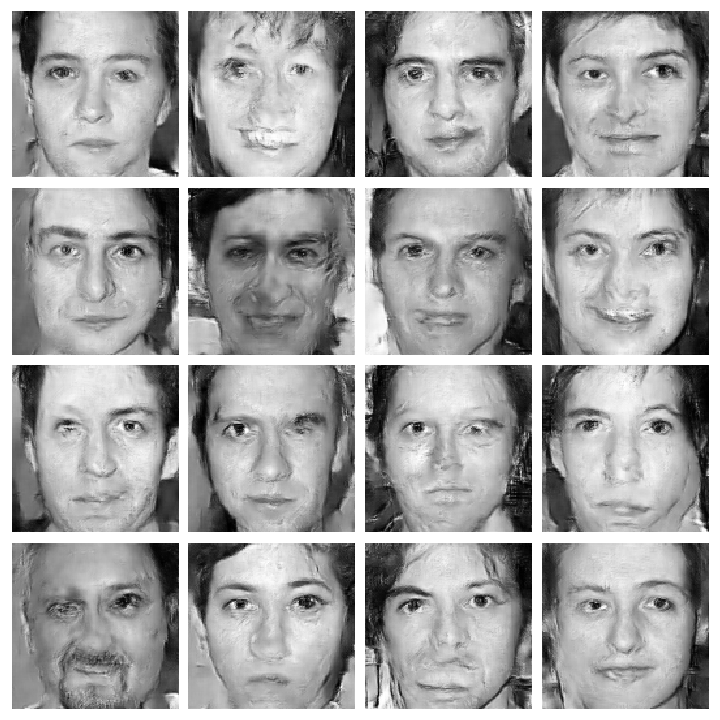
\includegraphics[width=\textwidth]{fig/dcgan/epoch4000}
%         \caption{Epoch 4000}
%     \end{subfigure}
%
%     \caption{Samples from DCGAN during traning on the Caltech dataset}
% \end{figure}
